\section{Introdução}


    Este trabalho apresenta um caso prático de sincronização de relógios usando o protocolo Network Time Protocol (NTP). O problema apresentado consiste em sincronizar as transições de estado de 4 semáforos de uma interseção sem que haja trocas de informações entre os eles. Deste modo, Todos os semáforos irão utilizar um relógio abstrato, escravizado de acordo com um servidor NTP, para inferir o seu estado (Verde, Vermelho).
    
    Por exemplo, considerando a figura \ref{fig:diagramaEstrada}, quando os semáforos da via horizontal (1 e 3) estão verdes, os via vertical (2 e 4) estão vermelhos. Ora, caso esta alteração de estado ocorra de $t$ em $t$ segundos, cada semáforo deve tomar essa decisão autonomamente de acordo com o seu relógio.
    Os quatro relógios apresentam características diferentes, pelo que $t$ segundo no semáforo 1 pode representar $t + \delta$ segundos no relógio 2, pelo que a transição no 2 seria tomada $\delta$ segundos mais tarde. Normalmente, $\delta$ é um valor muito pequeno, pelo que quando considerando uma só transição este valor é irrelevante. Contudo, esta discrepância acumula com o tempo e após duas transições já é de $2 \time \delta$, o que pode até levar ao caso de os dois semáforos estarem verdes ao mesmo tempo quando $N \times \delta = t$, em que $N$ é o número de transições ocorridas.
    A solução o problema é sincronizar os relógios do semáforos. Este processo não irá colocar $\delta$ a zero, mas sim mantê-lo com um valor baixo o suficiente para que seja irrelevante. Para tal. Cada semáforo irá atualizar periodicamente o "rate" e "offset" dos seus relógios com um servidor NTP, garantindo que $\delta$ não acumula infinitamente.  
    
    \begin{figure}[h]
        \centering
        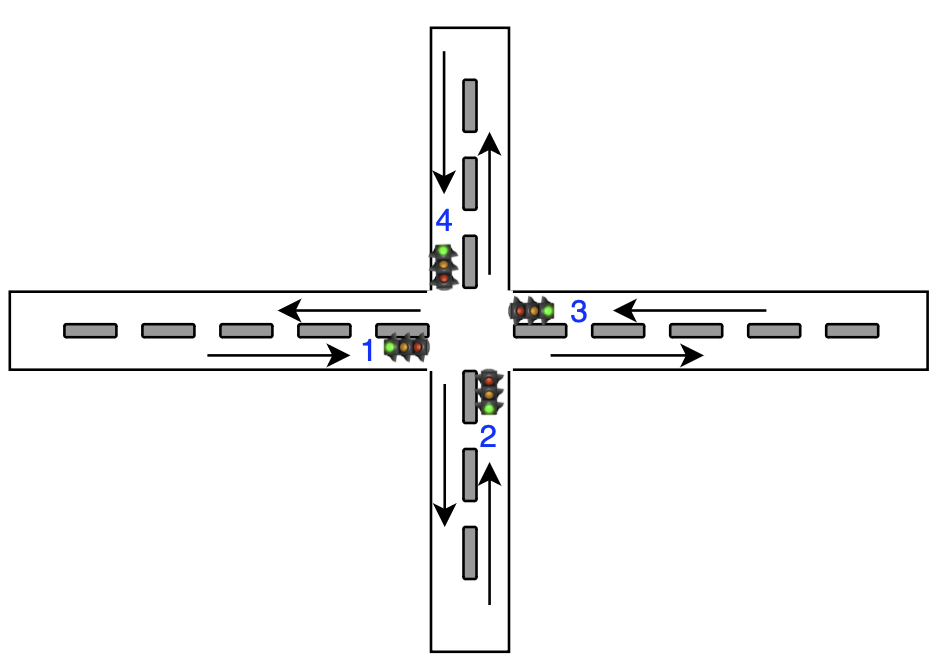
\includegraphics[width=0.8\linewidth]{figures/diagramaEstrada.png}
        \caption{Intresseção de uma estrada}
        \label{fig:diagramaEstrada}
    \end{figure}